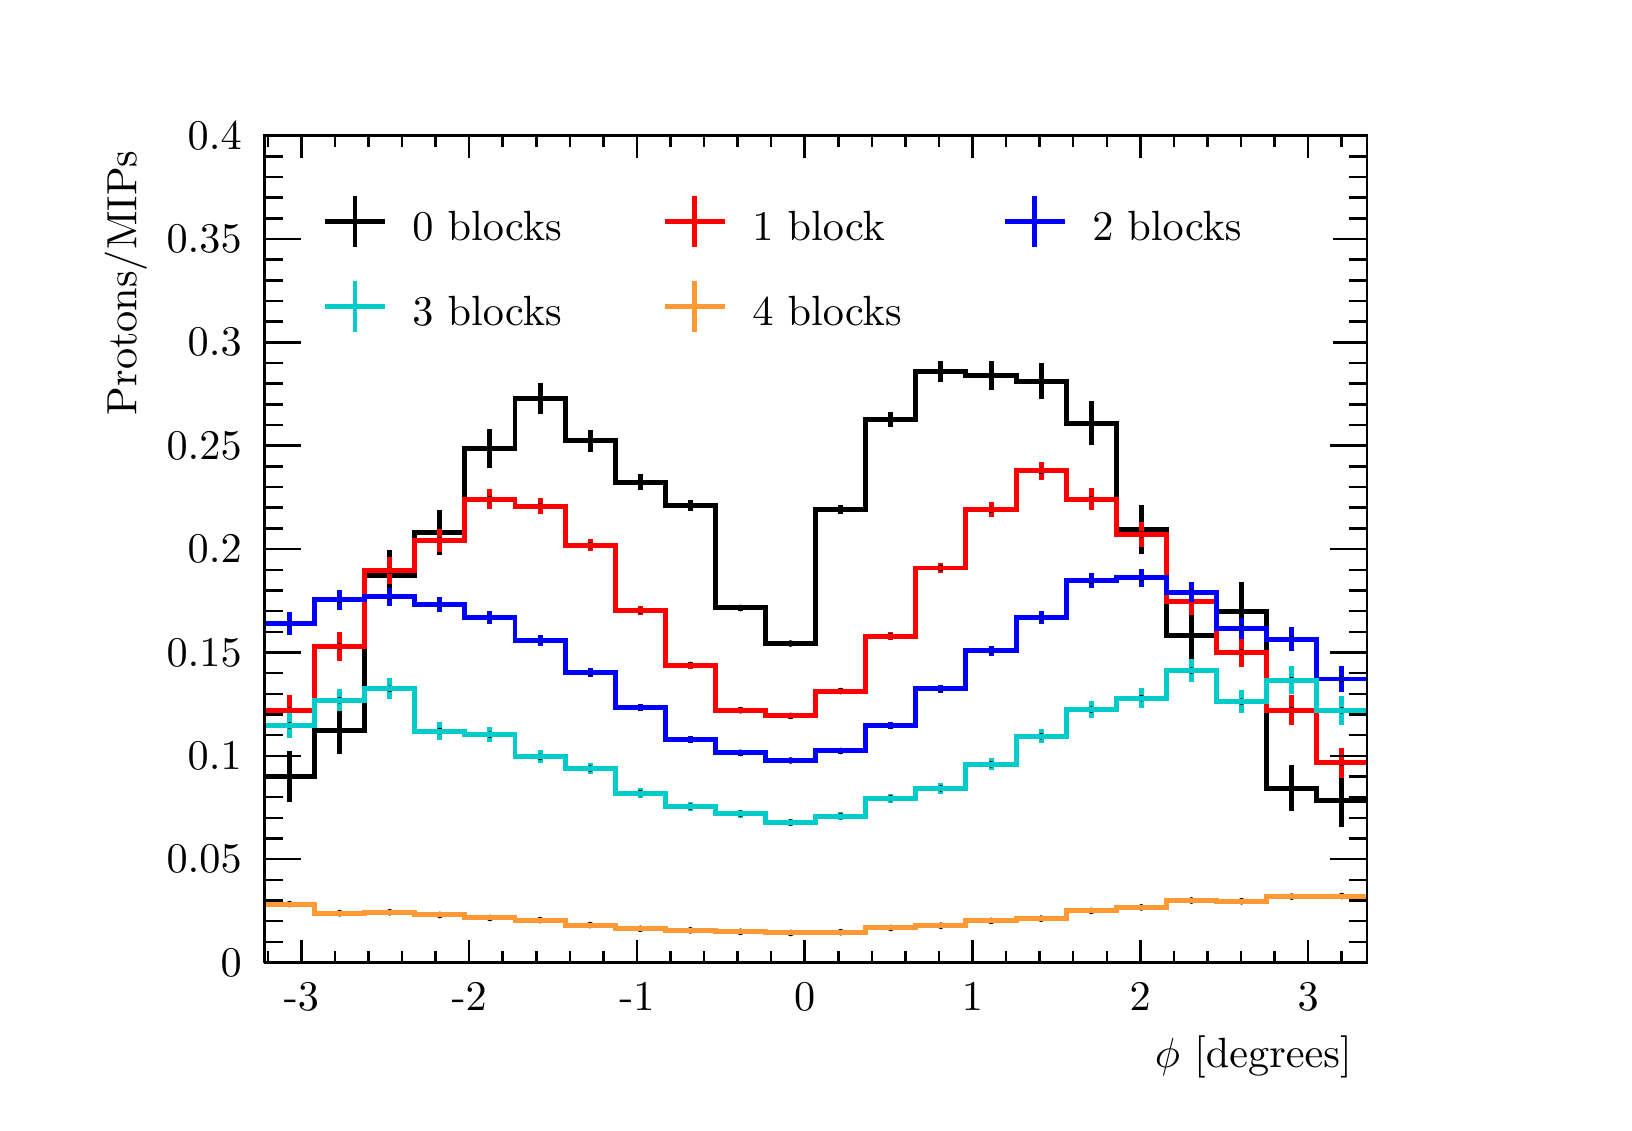
\begin{tikzpicture}
\pgfdeclareplotmark{cross} {
\pgfpathmoveto{\pgfpoint{-0.3\pgfplotmarksize}{\pgfplotmarksize}}
\pgfpathlineto{\pgfpoint{+0.3\pgfplotmarksize}{\pgfplotmarksize}}
\pgfpathlineto{\pgfpoint{+0.3\pgfplotmarksize}{0.3\pgfplotmarksize}}
\pgfpathlineto{\pgfpoint{+1\pgfplotmarksize}{0.3\pgfplotmarksize}}
\pgfpathlineto{\pgfpoint{+1\pgfplotmarksize}{-0.3\pgfplotmarksize}}
\pgfpathlineto{\pgfpoint{+0.3\pgfplotmarksize}{-0.3\pgfplotmarksize}}
\pgfpathlineto{\pgfpoint{+0.3\pgfplotmarksize}{-1.\pgfplotmarksize}}
\pgfpathlineto{\pgfpoint{-0.3\pgfplotmarksize}{-1.\pgfplotmarksize}}
\pgfpathlineto{\pgfpoint{-0.3\pgfplotmarksize}{-0.3\pgfplotmarksize}}
\pgfpathlineto{\pgfpoint{-1.\pgfplotmarksize}{-0.3\pgfplotmarksize}}
\pgfpathlineto{\pgfpoint{-1.\pgfplotmarksize}{0.3\pgfplotmarksize}}
\pgfpathlineto{\pgfpoint{-0.3\pgfplotmarksize}{0.3\pgfplotmarksize}}
\pgfpathclose
\pgfusepathqstroke
}
\pgfdeclareplotmark{cross*} {
\pgfpathmoveto{\pgfpoint{-0.3\pgfplotmarksize}{\pgfplotmarksize}}
\pgfpathlineto{\pgfpoint{+0.3\pgfplotmarksize}{\pgfplotmarksize}}
\pgfpathlineto{\pgfpoint{+0.3\pgfplotmarksize}{0.3\pgfplotmarksize}}
\pgfpathlineto{\pgfpoint{+1\pgfplotmarksize}{0.3\pgfplotmarksize}}
\pgfpathlineto{\pgfpoint{+1\pgfplotmarksize}{-0.3\pgfplotmarksize}}
\pgfpathlineto{\pgfpoint{+0.3\pgfplotmarksize}{-0.3\pgfplotmarksize}}
\pgfpathlineto{\pgfpoint{+0.3\pgfplotmarksize}{-1.\pgfplotmarksize}}
\pgfpathlineto{\pgfpoint{-0.3\pgfplotmarksize}{-1.\pgfplotmarksize}}
\pgfpathlineto{\pgfpoint{-0.3\pgfplotmarksize}{-0.3\pgfplotmarksize}}
\pgfpathlineto{\pgfpoint{-1.\pgfplotmarksize}{-0.3\pgfplotmarksize}}
\pgfpathlineto{\pgfpoint{-1.\pgfplotmarksize}{0.3\pgfplotmarksize}}
\pgfpathlineto{\pgfpoint{-0.3\pgfplotmarksize}{0.3\pgfplotmarksize}}
\pgfpathclose
\pgfusepathqfillstroke
}
\pgfdeclareplotmark{newstar} {
\pgfpathmoveto{\pgfqpoint{0pt}{\pgfplotmarksize}}
\pgfpathlineto{\pgfqpointpolar{44}{0.5\pgfplotmarksize}}
\pgfpathlineto{\pgfqpointpolar{18}{\pgfplotmarksize}}
\pgfpathlineto{\pgfqpointpolar{-20}{0.5\pgfplotmarksize}}
\pgfpathlineto{\pgfqpointpolar{-54}{\pgfplotmarksize}}
\pgfpathlineto{\pgfqpointpolar{-90}{0.5\pgfplotmarksize}}
\pgfpathlineto{\pgfqpointpolar{234}{\pgfplotmarksize}}
\pgfpathlineto{\pgfqpointpolar{198}{0.5\pgfplotmarksize}}
\pgfpathlineto{\pgfqpointpolar{162}{\pgfplotmarksize}}
\pgfpathlineto{\pgfqpointpolar{134}{0.5\pgfplotmarksize}}
\pgfpathclose
\pgfusepathqstroke
}
\pgfdeclareplotmark{newstar*} {
\pgfpathmoveto{\pgfqpoint{0pt}{\pgfplotmarksize}}
\pgfpathlineto{\pgfqpointpolar{44}{0.5\pgfplotmarksize}}
\pgfpathlineto{\pgfqpointpolar{18}{\pgfplotmarksize}}
\pgfpathlineto{\pgfqpointpolar{-20}{0.5\pgfplotmarksize}}
\pgfpathlineto{\pgfqpointpolar{-54}{\pgfplotmarksize}}
\pgfpathlineto{\pgfqpointpolar{-90}{0.5\pgfplotmarksize}}
\pgfpathlineto{\pgfqpointpolar{234}{\pgfplotmarksize}}
\pgfpathlineto{\pgfqpointpolar{198}{0.5\pgfplotmarksize}}
\pgfpathlineto{\pgfqpointpolar{162}{\pgfplotmarksize}}
\pgfpathlineto{\pgfqpointpolar{134}{0.5\pgfplotmarksize}}
\pgfpathclose
\pgfusepathqfillstroke
}
\definecolor{c}{rgb}{1,1,1};
\draw [color=c, fill=c] (0,0) rectangle (20,13.639);
\draw [color=c, fill=c] (3,1.77307) rectangle (17,12.2751);
\definecolor{c}{rgb}{0,0,0};
\draw [c,line width=0.9] (3,1.77307) -- (3,12.2751) -- (17,12.2751) -- (17,1.77307) -- (3,1.77307);
\definecolor{c}{rgb}{1,1,1};
\draw [color=c, fill=c] (3,1.77307) rectangle (17,12.2751);
\definecolor{c}{rgb}{0,0,0};
\draw [c,line width=0.9] (3,1.77307) -- (3,12.2751) -- (17,12.2751) -- (17,1.77307) -- (3,1.77307);
\draw [c,line width=0.9] (3,1.77307) -- (3.63636,1.77307) -- (3.63636,1.77307) -- (4.27273,1.77307) -- (4.27273,1.77307) -- (4.90909,1.77307) -- (4.90909,1.77307) -- (5.54545,1.77307) -- (5.54545,1.77307) -- (6.18182,1.77307) -- (6.18182,1.77307) --
 (6.81818,1.77307) -- (6.81818,1.77307) -- (7.45455,1.77307) -- (7.45455,1.77307) -- (8.09091,1.77307) -- (8.09091,1.77307) -- (8.72727,1.77307) -- (8.72727,1.77307) -- (9.36364,1.77307) -- (9.36364,1.77307) -- (10,1.77307) -- (10,1.77307) --
 (10.6364,1.77307) -- (10.6364,1.77307) -- (11.2727,1.77307) -- (11.2727,1.77307) -- (11.9091,1.77307) -- (11.9091,1.77307) -- (12.5455,1.77307) -- (12.5455,1.77307) -- (13.1818,1.77307) -- (13.1818,1.77307) -- (13.8182,1.77307) -- (13.8182,1.77307)
 -- (14.4545,1.77307) -- (14.4545,1.77307) -- (15.0909,1.77307) -- (15.0909,1.77307) -- (15.7273,1.77307) -- (15.7273,1.77307) -- (16.3636,1.77307) -- (16.3636,1.77307) -- (17,1.77307);
\draw [c,line width=0.9] (3,1.77307) -- (17,1.77307);
\draw [c,line width=0.9] (3.4688,2.05948) -- (3.4688,1.77307);
\draw [c,line width=0.9] (3.89498,1.91628) -- (3.89498,1.77307);
\draw [c,line width=0.9] (4.32116,1.91628) -- (4.32116,1.77307);
\draw [c,line width=0.9] (4.74734,1.91628) -- (4.74734,1.77307);
\draw [c,line width=0.9] (5.17352,1.91628) -- (5.17352,1.77307);
\draw [c,line width=0.9] (5.5997,2.05948) -- (5.5997,1.77307);
\draw [c,line width=0.9] (6.02588,1.91628) -- (6.02588,1.77307);
\draw [c,line width=0.9] (6.45205,1.91628) -- (6.45205,1.77307);
\draw [c,line width=0.9] (6.87823,1.91628) -- (6.87823,1.77307);
\draw [c,line width=0.9] (7.30441,1.91628) -- (7.30441,1.77307);
\draw [c,line width=0.9] (7.73059,2.05948) -- (7.73059,1.77307);
\draw [c,line width=0.9] (8.15677,1.91628) -- (8.15677,1.77307);
\draw [c,line width=0.9] (8.58295,1.91628) -- (8.58295,1.77307);
\draw [c,line width=0.9] (9.00913,1.91628) -- (9.00913,1.77307);
\draw [c,line width=0.9] (9.43531,1.91628) -- (9.43531,1.77307);
\draw [c,line width=0.9] (9.86149,2.05948) -- (9.86149,1.77307);
\draw [c,line width=0.9] (10.2877,1.91628) -- (10.2877,1.77307);
\draw [c,line width=0.9] (10.7139,1.91628) -- (10.7139,1.77307);
\draw [c,line width=0.9] (11.14,1.91628) -- (11.14,1.77307);
\draw [c,line width=0.9] (11.5662,1.91628) -- (11.5662,1.77307);
\draw [c,line width=0.9] (11.9924,2.05948) -- (11.9924,1.77307);
\draw [c,line width=0.9] (12.4186,1.91628) -- (12.4186,1.77307);
\draw [c,line width=0.9] (12.8447,1.91628) -- (12.8447,1.77307);
\draw [c,line width=0.9] (13.2709,1.91628) -- (13.2709,1.77307);
\draw [c,line width=0.9] (13.6971,1.91628) -- (13.6971,1.77307);
\draw [c,line width=0.9] (14.1233,2.05948) -- (14.1233,1.77307);
\draw [c,line width=0.9] (14.5495,1.91628) -- (14.5495,1.77307);
\draw [c,line width=0.9] (14.9756,1.91628) -- (14.9756,1.77307);
\draw [c,line width=0.9] (15.4018,1.91628) -- (15.4018,1.77307);
\draw [c,line width=0.9] (15.828,1.91628) -- (15.828,1.77307);
\draw [c,line width=0.9] (16.2542,2.05948) -- (16.2542,1.77307);
\draw [c,line width=0.9] (3.4688,2.05948) -- (3.4688,1.77307);
\draw [c,line width=0.9] (3.04262,1.91628) -- (3.04262,1.77307);
\draw [c,line width=0.9] (16.2542,2.05948) -- (16.2542,1.77307);
\draw [c,line width=0.9] (16.6804,1.91628) -- (16.6804,1.77307);
\draw [anchor=base] (3.4688,1.15931) node[scale=1.52731, color=c, rotate=0]{-3};
\draw [anchor=base] (5.5997,1.15931) node[scale=1.52731, color=c, rotate=0]{-2};
\draw [anchor=base] (7.73059,1.15931) node[scale=1.52731, color=c, rotate=0]{-1};
\draw [anchor=base] (9.86149,1.15931) node[scale=1.52731, color=c, rotate=0]{0};
\draw [anchor=base] (11.9924,1.15931) node[scale=1.52731, color=c, rotate=0]{1};
\draw [anchor=base] (14.1233,1.15931) node[scale=1.52731, color=c, rotate=0]{2};
\draw [anchor=base] (16.2542,1.15931) node[scale=1.52731, color=c, rotate=0]{3};
\draw [anchor= east] (17,0.572837) node[scale=1.52731, color=c, rotate=0]{$\phi$ [degrees]};
\draw [c,line width=0.9] (3,12.2751) -- (17,12.2751);
\draw [c,line width=0.9] (3.4688,11.9887) -- (3.4688,12.2751);
\draw [c,line width=0.9] (3.89498,12.1319) -- (3.89498,12.2751);
\draw [c,line width=0.9] (4.32116,12.1319) -- (4.32116,12.2751);
\draw [c,line width=0.9] (4.74734,12.1319) -- (4.74734,12.2751);
\draw [c,line width=0.9] (5.17352,12.1319) -- (5.17352,12.2751);
\draw [c,line width=0.9] (5.5997,11.9887) -- (5.5997,12.2751);
\draw [c,line width=0.9] (6.02588,12.1319) -- (6.02588,12.2751);
\draw [c,line width=0.9] (6.45205,12.1319) -- (6.45205,12.2751);
\draw [c,line width=0.9] (6.87823,12.1319) -- (6.87823,12.2751);
\draw [c,line width=0.9] (7.30441,12.1319) -- (7.30441,12.2751);
\draw [c,line width=0.9] (7.73059,11.9887) -- (7.73059,12.2751);
\draw [c,line width=0.9] (8.15677,12.1319) -- (8.15677,12.2751);
\draw [c,line width=0.9] (8.58295,12.1319) -- (8.58295,12.2751);
\draw [c,line width=0.9] (9.00913,12.1319) -- (9.00913,12.2751);
\draw [c,line width=0.9] (9.43531,12.1319) -- (9.43531,12.2751);
\draw [c,line width=0.9] (9.86149,11.9887) -- (9.86149,12.2751);
\draw [c,line width=0.9] (10.2877,12.1319) -- (10.2877,12.2751);
\draw [c,line width=0.9] (10.7139,12.1319) -- (10.7139,12.2751);
\draw [c,line width=0.9] (11.14,12.1319) -- (11.14,12.2751);
\draw [c,line width=0.9] (11.5662,12.1319) -- (11.5662,12.2751);
\draw [c,line width=0.9] (11.9924,11.9887) -- (11.9924,12.2751);
\draw [c,line width=0.9] (12.4186,12.1319) -- (12.4186,12.2751);
\draw [c,line width=0.9] (12.8447,12.1319) -- (12.8447,12.2751);
\draw [c,line width=0.9] (13.2709,12.1319) -- (13.2709,12.2751);
\draw [c,line width=0.9] (13.6971,12.1319) -- (13.6971,12.2751);
\draw [c,line width=0.9] (14.1233,11.9887) -- (14.1233,12.2751);
\draw [c,line width=0.9] (14.5495,12.1319) -- (14.5495,12.2751);
\draw [c,line width=0.9] (14.9756,12.1319) -- (14.9756,12.2751);
\draw [c,line width=0.9] (15.4018,12.1319) -- (15.4018,12.2751);
\draw [c,line width=0.9] (15.828,12.1319) -- (15.828,12.2751);
\draw [c,line width=0.9] (16.2542,11.9887) -- (16.2542,12.2751);
\draw [c,line width=0.9] (3.4688,11.9887) -- (3.4688,12.2751);
\draw [c,line width=0.9] (3.04262,12.1319) -- (3.04262,12.2751);
\draw [c,line width=0.9] (16.2542,11.9887) -- (16.2542,12.2751);
\draw [c,line width=0.9] (16.6804,12.1319) -- (16.6804,12.2751);
\draw [c,line width=0.9] (3,1.77307) -- (3,12.2751);
\draw [c,line width=0.9] (3.462,1.77307) -- (3,1.77307);
\draw [c,line width=0.9] (3.231,2.03562) -- (3,2.03562);
\draw [c,line width=0.9] (3.231,2.29817) -- (3,2.29817);
\draw [c,line width=0.9] (3.231,2.56072) -- (3,2.56072);
\draw [c,line width=0.9] (3.231,2.82327) -- (3,2.82327);
\draw [c,line width=0.9] (3.462,3.08582) -- (3,3.08582);
\draw [c,line width=0.9] (3.231,3.34837) -- (3,3.34837);
\draw [c,line width=0.9] (3.231,3.61092) -- (3,3.61092);
\draw [c,line width=0.9] (3.231,3.87347) -- (3,3.87347);
\draw [c,line width=0.9] (3.231,4.13602) -- (3,4.13602);
\draw [c,line width=0.9] (3.462,4.39857) -- (3,4.39857);
\draw [c,line width=0.9] (3.231,4.66112) -- (3,4.66112);
\draw [c,line width=0.9] (3.231,4.92367) -- (3,4.92367);
\draw [c,line width=0.9] (3.231,5.18622) -- (3,5.18622);
\draw [c,line width=0.9] (3.231,5.44877) -- (3,5.44877);
\draw [c,line width=0.9] (3.462,5.71132) -- (3,5.71132);
\draw [c,line width=0.9] (3.231,5.97387) -- (3,5.97387);
\draw [c,line width=0.9] (3.231,6.23642) -- (3,6.23642);
\draw [c,line width=0.9] (3.231,6.49897) -- (3,6.49897);
\draw [c,line width=0.9] (3.231,6.76152) -- (3,6.76152);
\draw [c,line width=0.9] (3.462,7.02407) -- (3,7.02407);
\draw [c,line width=0.9] (3.231,7.28662) -- (3,7.28662);
\draw [c,line width=0.9] (3.231,7.54917) -- (3,7.54917);
\draw [c,line width=0.9] (3.231,7.81172) -- (3,7.81172);
\draw [c,line width=0.9] (3.231,8.07427) -- (3,8.07427);
\draw [c,line width=0.9] (3.462,8.33682) -- (3,8.33682);
\draw [c,line width=0.9] (3.231,8.59937) -- (3,8.59937);
\draw [c,line width=0.9] (3.231,8.86192) -- (3,8.86192);
\draw [c,line width=0.9] (3.231,9.12447) -- (3,9.12447);
\draw [c,line width=0.9] (3.231,9.38702) -- (3,9.38702);
\draw [c,line width=0.9] (3.462,9.64957) -- (3,9.64957);
\draw [c,line width=0.9] (3.231,9.91212) -- (3,9.91212);
\draw [c,line width=0.9] (3.231,10.1747) -- (3,10.1747);
\draw [c,line width=0.9] (3.231,10.4372) -- (3,10.4372);
\draw [c,line width=0.9] (3.231,10.6998) -- (3,10.6998);
\draw [c,line width=0.9] (3.462,10.9623) -- (3,10.9623);
\draw [c,line width=0.9] (3.231,11.2249) -- (3,11.2249);
\draw [c,line width=0.9] (3.231,11.4874) -- (3,11.4874);
\draw [c,line width=0.9] (3.231,11.75) -- (3,11.75);
\draw [c,line width=0.9] (3.231,12.0125) -- (3,12.0125);
\draw [c,line width=0.9] (3.462,12.2751) -- (3,12.2751);
\draw [anchor= east] (2.9,1.77307) node[scale=1.52731, color=c, rotate=0]{0};
\draw [anchor= east] (2.9,3.08582) node[scale=1.52731, color=c, rotate=0]{0.05};
\draw [anchor= east] (2.9,4.39857) node[scale=1.52731, color=c, rotate=0]{0.1};
\draw [anchor= east] (2.9,5.71132) node[scale=1.52731, color=c, rotate=0]{0.15};
\draw [anchor= east] (2.9,7.02407) node[scale=1.52731, color=c, rotate=0]{0.2};
\draw [anchor= east] (2.9,8.33682) node[scale=1.52731, color=c, rotate=0]{0.25};
\draw [anchor= east] (2.9,9.64957) node[scale=1.52731, color=c, rotate=0]{0.3};
\draw [anchor= east] (2.9,10.9623) node[scale=1.52731, color=c, rotate=0]{0.35};
\draw [anchor= east] (2.9,12.2751) node[scale=1.52731, color=c, rotate=0]{0.4};
\draw [anchor= east] (1.24,12.2751) node[scale=1.52731, color=c, rotate=90]{  Protons/MIPs};
\draw [c,line width=0.9] (17,1.77307) -- (17,12.2751);
\draw [c,line width=0.9] (16.538,1.77307) -- (17,1.77307);
\draw [c,line width=0.9] (16.769,2.03562) -- (17,2.03562);
\draw [c,line width=0.9] (16.769,2.29817) -- (17,2.29817);
\draw [c,line width=0.9] (16.769,2.56072) -- (17,2.56072);
\draw [c,line width=0.9] (16.769,2.82327) -- (17,2.82327);
\draw [c,line width=0.9] (16.538,3.08582) -- (17,3.08582);
\draw [c,line width=0.9] (16.769,3.34837) -- (17,3.34837);
\draw [c,line width=0.9] (16.769,3.61092) -- (17,3.61092);
\draw [c,line width=0.9] (16.769,3.87347) -- (17,3.87347);
\draw [c,line width=0.9] (16.769,4.13602) -- (17,4.13602);
\draw [c,line width=0.9] (16.538,4.39857) -- (17,4.39857);
\draw [c,line width=0.9] (16.769,4.66112) -- (17,4.66112);
\draw [c,line width=0.9] (16.769,4.92367) -- (17,4.92367);
\draw [c,line width=0.9] (16.769,5.18622) -- (17,5.18622);
\draw [c,line width=0.9] (16.769,5.44877) -- (17,5.44877);
\draw [c,line width=0.9] (16.538,5.71132) -- (17,5.71132);
\draw [c,line width=0.9] (16.769,5.97387) -- (17,5.97387);
\draw [c,line width=0.9] (16.769,6.23642) -- (17,6.23642);
\draw [c,line width=0.9] (16.769,6.49897) -- (17,6.49897);
\draw [c,line width=0.9] (16.769,6.76152) -- (17,6.76152);
\draw [c,line width=0.9] (16.538,7.02407) -- (17,7.02407);
\draw [c,line width=0.9] (16.769,7.28662) -- (17,7.28662);
\draw [c,line width=0.9] (16.769,7.54917) -- (17,7.54917);
\draw [c,line width=0.9] (16.769,7.81172) -- (17,7.81172);
\draw [c,line width=0.9] (16.769,8.07427) -- (17,8.07427);
\draw [c,line width=0.9] (16.538,8.33682) -- (17,8.33682);
\draw [c,line width=0.9] (16.769,8.59937) -- (17,8.59937);
\draw [c,line width=0.9] (16.769,8.86192) -- (17,8.86192);
\draw [c,line width=0.9] (16.769,9.12447) -- (17,9.12447);
\draw [c,line width=0.9] (16.769,9.38702) -- (17,9.38702);
\draw [c,line width=0.9] (16.538,9.64957) -- (17,9.64957);
\draw [c,line width=0.9] (16.769,9.91212) -- (17,9.91212);
\draw [c,line width=0.9] (16.769,10.1747) -- (17,10.1747);
\draw [c,line width=0.9] (16.769,10.4372) -- (17,10.4372);
\draw [c,line width=0.9] (16.769,10.6998) -- (17,10.6998);
\draw [c,line width=0.9] (16.538,10.9623) -- (17,10.9623);
\draw [c,line width=0.9] (16.769,11.2249) -- (17,11.2249);
\draw [c,line width=0.9] (16.769,11.4874) -- (17,11.4874);
\draw [c,line width=0.9] (16.769,11.75) -- (17,11.75);
\draw [c,line width=0.9] (16.769,12.0125) -- (17,12.0125);
\draw [c,line width=0.9] (16.538,12.2751) -- (17,12.2751);
\draw [c,line width=1.8] (3.31818,3.80808) -- (3.31818,4.13307);
\draw [c,line width=1.8] (3.31818,4.13307) -- (3.31818,4.45805);
\foreach \P in {(3.31818,4.13307)}{\draw[mark options={color=c,fill=c},mark size=2.402402pt,mark=*,mark size=1pt] plot coordinates {\P};}
\draw [c,line width=1.8] (3.95455,4.41539) -- (3.95455,4.72226);
\draw [c,line width=1.8] (3.95455,4.72226) -- (3.95455,5.02913);
\foreach \P in {(3.95455,4.72226)}{\draw[mark options={color=c,fill=c},mark size=2.402402pt,mark=*,mark size=1pt] plot coordinates {\P};}
\draw [c,line width=1.8] (4.59091,6.36336) -- (4.59091,6.68924);
\draw [c,line width=1.8] (4.59091,6.68924) -- (4.59091,7.01511);
\foreach \P in {(4.59091,6.68924)}{\draw[mark options={color=c,fill=c},mark size=2.402402pt,mark=*,mark size=1pt] plot coordinates {\P};}
\draw [c,line width=1.8] (5.22727,6.95027) -- (5.22727,7.23731);
\draw [c,line width=1.8] (5.22727,7.23731) -- (5.22727,7.52435);
\foreach \P in {(5.22727,7.23731)}{\draw[mark options={color=c,fill=c},mark size=2.402402pt,mark=*,mark size=1pt] plot coordinates {\P};}
\draw [c,line width=1.8] (5.86364,8.05935) -- (5.86364,8.30108);
\draw [c,line width=1.8] (5.86364,8.30108) -- (5.86364,8.54282);
\foreach \P in {(5.86364,8.30108)}{\draw[mark options={color=c,fill=c},mark size=2.402402pt,mark=*,mark size=1pt] plot coordinates {\P};}
\draw [c,line width=1.8] (6.5,8.738) -- (6.5,8.93286);
\draw [c,line width=1.8] (6.5,8.93286) -- (6.5,9.12772);
\foreach \P in {(6.5,8.93286)}{\draw[mark options={color=c,fill=c},mark size=2.402402pt,mark=*,mark size=1pt] plot coordinates {\P};}
\draw [c,line width=1.8] (7.13636,8.25921) -- (7.13636,8.39849);
\draw [c,line width=1.8] (7.13636,8.39849) -- (7.13636,8.53777);
\foreach \P in {(7.13636,8.39849)}{\draw[mark options={color=c,fill=c},mark size=2.402402pt,mark=*,mark size=1pt] plot coordinates {\P};}
\draw [c,line width=1.8] (7.77273,7.77828) -- (7.77273,7.87577);
\draw [c,line width=1.8] (7.77273,7.87577) -- (7.77273,7.97326);
\foreach \P in {(7.77273,7.87577)}{\draw[mark options={color=c,fill=c},mark size=2.402402pt,mark=*,mark size=1pt] plot coordinates {\P};}
\draw [c,line width=1.8] (8.40909,7.5099) -- (8.40909,7.57818);
\draw [c,line width=1.8] (8.40909,7.57818) -- (8.40909,7.64647);
\foreach \P in {(8.40909,7.57818)}{\draw[mark options={color=c,fill=c},mark size=2.402402pt,mark=*,mark size=1pt] plot coordinates {\P};}
\draw [c,line width=1.8] (9.04545,6.23857) -- (9.04545,6.27671);
\draw [c,line width=1.8] (9.04545,6.27671) -- (9.04545,6.31485);
\foreach \P in {(9.04545,6.27671)}{\draw[mark options={color=c,fill=c},mark size=2.402402pt,mark=*,mark size=1pt] plot coordinates {\P};}
\draw [c,line width=1.8] (9.68182,5.79204) -- (9.68182,5.82443);
\draw [c,line width=1.8] (9.68182,5.82443) -- (9.68182,5.85681);
\foreach \P in {(9.68182,5.82443)}{\draw[mark options={color=c,fill=c},mark size=2.402402pt,mark=*,mark size=1pt] plot coordinates {\P};}
\draw [c,line width=1.8] (10.3182,7.47425) -- (10.3182,7.53112);
\draw [c,line width=1.8] (10.3182,7.53112) -- (10.3182,7.58798);
\foreach \P in {(10.3182,7.53112)}{\draw[mark options={color=c,fill=c},mark size=2.402402pt,mark=*,mark size=1pt] plot coordinates {\P};}
\draw [c,line width=1.8] (10.9545,8.57392) -- (10.9545,8.66757);
\draw [c,line width=1.8] (10.9545,8.66757) -- (10.9545,8.76122);
\foreach \P in {(10.9545,8.66757)}{\draw[mark options={color=c,fill=c},mark size=2.402402pt,mark=*,mark size=1pt] plot coordinates {\P};}
\draw [c,line width=1.8] (11.5909,9.14225) -- (11.5909,9.27642);
\draw [c,line width=1.8] (11.5909,9.27642) -- (11.5909,9.41059);
\foreach \P in {(11.5909,9.27642)}{\draw[mark options={color=c,fill=c},mark size=2.402402pt,mark=*,mark size=1pt] plot coordinates {\P};}
\draw [c,line width=1.8] (12.2273,9.04159) -- (12.2273,9.22441);
\draw [c,line width=1.8] (12.2273,9.22441) -- (12.2273,9.40722);
\foreach \P in {(12.2273,9.22441)}{\draw[mark options={color=c,fill=c},mark size=2.402402pt,mark=*,mark size=1pt] plot coordinates {\P};}
\draw [c,line width=1.8] (12.8636,8.92559) -- (12.8636,9.15666);
\draw [c,line width=1.8] (12.8636,9.15666) -- (12.8636,9.38773);
\foreach \P in {(12.8636,9.15666)}{\draw[mark options={color=c,fill=c},mark size=2.402402pt,mark=*,mark size=1pt] plot coordinates {\P};}
\draw [c,line width=1.8] (13.5,8.34016) -- (13.5,8.62085);
\draw [c,line width=1.8] (13.5,8.62085) -- (13.5,8.90154);
\foreach \P in {(13.5,8.62085)}{\draw[mark options={color=c,fill=c},mark size=2.402402pt,mark=*,mark size=1pt] plot coordinates {\P};}
\draw [c,line width=1.8] (14.1364,6.96408) -- (14.1364,7.27082);
\draw [c,line width=1.8] (14.1364,7.27082) -- (14.1364,7.57756);
\foreach \P in {(14.1364,7.27082)}{\draw[mark options={color=c,fill=c},mark size=2.402402pt,mark=*,mark size=1pt] plot coordinates {\P};}
\draw [c,line width=1.8] (14.7727,5.6213) -- (14.7727,5.92854);
\draw [c,line width=1.8] (14.7727,5.92854) -- (14.7727,6.23577);
\foreach \P in {(14.7727,5.92854)}{\draw[mark options={color=c,fill=c},mark size=2.402402pt,mark=*,mark size=1pt] plot coordinates {\P};}
\draw [c,line width=1.8] (15.4091,5.86537) -- (15.4091,6.23494);
\draw [c,line width=1.8] (15.4091,6.23494) -- (15.4091,6.60452);
\foreach \P in {(15.4091,6.23494)}{\draw[mark options={color=c,fill=c},mark size=2.402402pt,mark=*,mark size=1pt] plot coordinates {\P};}
\draw [c,line width=1.8] (16.0455,3.69529) -- (16.0455,3.9894);
\draw [c,line width=1.8] (16.0455,3.9894) -- (16.0455,4.28351);
\foreach \P in {(16.0455,3.9894)}{\draw[mark options={color=c,fill=c},mark size=2.402402pt,mark=*,mark size=1pt] plot coordinates {\P};}
\draw [c,line width=1.8] (16.6818,3.49909) -- (16.6818,3.83344);
\draw [c,line width=1.8] (16.6818,3.83344) -- (16.6818,4.16778);
\foreach \P in {(16.6818,3.83344)}{\draw[mark options={color=c,fill=c},mark size=2.402402pt,mark=*,mark size=1pt] plot coordinates {\P};}
\draw [c,line width=1.8] (3,4.13307) -- (3.63636,4.13307) -- (3.63636,4.72226) -- (4.27273,4.72226) -- (4.27273,6.68924) -- (4.90909,6.68924) -- (4.90909,7.23731) -- (5.54545,7.23731) -- (5.54545,8.30108) -- (6.18182,8.30108) -- (6.18182,8.93286) --
 (6.81818,8.93286) -- (6.81818,8.39849) -- (7.45455,8.39849) -- (7.45455,7.87577) -- (8.09091,7.87577) -- (8.09091,7.57818) -- (8.72727,7.57818) -- (8.72727,6.27671) -- (9.36364,6.27671) -- (9.36364,5.82443) -- (10,5.82443) -- (10,7.53112) --
 (10.6364,7.53112) -- (10.6364,8.66757) -- (11.2727,8.66757) -- (11.2727,9.27642) -- (11.9091,9.27642) -- (11.9091,9.22441) -- (12.5455,9.22441) -- (12.5455,9.15666) -- (13.1818,9.15666) -- (13.1818,8.62085) -- (13.8182,8.62085) -- (13.8182,7.27082)
 -- (14.4545,7.27082) -- (14.4545,5.92854) -- (15.0909,5.92854) -- (15.0909,6.23494) -- (15.7273,6.23494) -- (15.7273,3.9894) -- (16.3636,3.9894) -- (16.3636,3.83344) -- (17,3.83344);
\definecolor{c}{rgb}{1,0,0};
\draw [c,line width=1.8] (3.31818,4.78145) -- (3.31818,4.97313);
\draw [c,line width=1.8] (3.31818,4.97313) -- (3.31818,5.16481);
\definecolor{c}{rgb}{0,0,0};
\foreach \P in {(3.31818,4.97313)}{\draw[mark options={color=c,fill=c},mark size=2.402402pt,mark=*,mark size=1pt] plot coordinates {\P};}
\definecolor{c}{rgb}{1,0,0};
\draw [c,line width=1.8] (3.95455,5.6081) -- (3.95455,5.78705);
\draw [c,line width=1.8] (3.95455,5.78705) -- (3.95455,5.96599);
\definecolor{c}{rgb}{0,0,0};
\foreach \P in {(3.95455,5.78705)}{\draw[mark options={color=c,fill=c},mark size=2.402402pt,mark=*,mark size=1pt] plot coordinates {\P};}
\definecolor{c}{rgb}{1,0,0};
\draw [c,line width=1.8] (4.59091,6.57712) -- (4.59091,6.74842);
\draw [c,line width=1.8] (4.59091,6.74842) -- (4.59091,6.91972);
\definecolor{c}{rgb}{0,0,0};
\foreach \P in {(4.59091,6.74842)}{\draw[mark options={color=c,fill=c},mark size=2.402402pt,mark=*,mark size=1pt] plot coordinates {\P};}
\definecolor{c}{rgb}{1,0,0};
\draw [c,line width=1.8] (5.22727,6.98706) -- (5.22727,7.13564);
\draw [c,line width=1.8] (5.22727,7.13564) -- (5.22727,7.28422);
\definecolor{c}{rgb}{0,0,0};
\foreach \P in {(5.22727,7.13564)}{\draw[mark options={color=c,fill=c},mark size=2.402402pt,mark=*,mark size=1pt] plot coordinates {\P};}
\definecolor{c}{rgb}{1,0,0};
\draw [c,line width=1.8] (5.86364,7.53021) -- (5.86364,7.65829);
\draw [c,line width=1.8] (5.86364,7.65829) -- (5.86364,7.78638);
\definecolor{c}{rgb}{0,0,0};
\foreach \P in {(5.86364,7.65829)}{\draw[mark options={color=c,fill=c},mark size=2.402402pt,mark=*,mark size=1pt] plot coordinates {\P};}
\definecolor{c}{rgb}{1,0,0};
\draw [c,line width=1.8] (6.5,7.46591) -- (6.5,7.5684);
\draw [c,line width=1.8] (6.5,7.5684) -- (6.5,7.67089);
\definecolor{c}{rgb}{0,0,0};
\foreach \P in {(6.5,7.5684)}{\draw[mark options={color=c,fill=c},mark size=2.402402pt,mark=*,mark size=1pt] plot coordinates {\P};}
\definecolor{c}{rgb}{1,0,0};
\draw [c,line width=1.8] (7.13636,6.99514) -- (7.13636,7.07247);
\draw [c,line width=1.8] (7.13636,7.07247) -- (7.13636,7.14981);
\definecolor{c}{rgb}{0,0,0};
\foreach \P in {(7.13636,7.07247)}{\draw[mark options={color=c,fill=c},mark size=2.402402pt,mark=*,mark size=1pt] plot coordinates {\P};}
\definecolor{c}{rgb}{1,0,0};
\draw [c,line width=1.8] (7.77273,6.18448) -- (7.77273,6.24109);
\draw [c,line width=1.8] (7.77273,6.24109) -- (7.77273,6.29769);
\definecolor{c}{rgb}{0,0,0};
\foreach \P in {(7.77273,6.24109)}{\draw[mark options={color=c,fill=c},mark size=2.402402pt,mark=*,mark size=1pt] plot coordinates {\P};}
\definecolor{c}{rgb}{1,0,0};
\draw [c,line width=1.8] (8.40909,5.5071) -- (8.40909,5.55116);
\draw [c,line width=1.8] (8.40909,5.55116) -- (8.40909,5.59522);
\definecolor{c}{rgb}{0,0,0};
\foreach \P in {(8.40909,5.55116)}{\draw[mark options={color=c,fill=c},mark size=2.402402pt,mark=*,mark size=1pt] plot coordinates {\P};}
\definecolor{c}{rgb}{1,0,0};
\draw [c,line width=1.8] (9.04545,4.94121) -- (9.04545,4.97695);
\draw [c,line width=1.8] (9.04545,4.97695) -- (9.04545,5.01268);
\definecolor{c}{rgb}{0,0,0};
\foreach \P in {(9.04545,4.97695)}{\draw[mark options={color=c,fill=c},mark size=2.402402pt,mark=*,mark size=1pt] plot coordinates {\P};}
\definecolor{c}{rgb}{1,0,0};
\draw [c,line width=1.8] (9.68182,4.87123) -- (9.68182,4.9057);
\draw [c,line width=1.8] (9.68182,4.9057) -- (9.68182,4.94017);
\definecolor{c}{rgb}{0,0,0};
\foreach \P in {(9.68182,4.9057)}{\draw[mark options={color=c,fill=c},mark size=2.402402pt,mark=*,mark size=1pt] plot coordinates {\P};}
\definecolor{c}{rgb}{1,0,0};
\draw [c,line width=1.8] (10.3182,5.18155) -- (10.3182,5.22031);
\draw [c,line width=1.8] (10.3182,5.22031) -- (10.3182,5.25907);
\definecolor{c}{rgb}{0,0,0};
\foreach \P in {(10.3182,5.22031)}{\draw[mark options={color=c,fill=c},mark size=2.402402pt,mark=*,mark size=1pt] plot coordinates {\P};}
\definecolor{c}{rgb}{1,0,0};
\draw [c,line width=1.8] (10.9545,5.86661) -- (10.9545,5.91603);
\draw [c,line width=1.8] (10.9545,5.91603) -- (10.9545,5.96545);
\definecolor{c}{rgb}{0,0,0};
\foreach \P in {(10.9545,5.91603)}{\draw[mark options={color=c,fill=c},mark size=2.402402pt,mark=*,mark size=1pt] plot coordinates {\P};}
\definecolor{c}{rgb}{1,0,0};
\draw [c,line width=1.8] (11.5909,6.71715) -- (11.5909,6.78377);
\draw [c,line width=1.8] (11.5909,6.78377) -- (11.5909,6.85039);
\definecolor{c}{rgb}{0,0,0};
\foreach \P in {(11.5909,6.78377)}{\draw[mark options={color=c,fill=c},mark size=2.402402pt,mark=*,mark size=1pt] plot coordinates {\P};}
\definecolor{c}{rgb}{1,0,0};
\draw [c,line width=1.8] (12.2273,7.43032) -- (12.2273,7.52302);
\draw [c,line width=1.8] (12.2273,7.52302) -- (12.2273,7.61572);
\definecolor{c}{rgb}{0,0,0};
\foreach \P in {(12.2273,7.52302)}{\draw[mark options={color=c,fill=c},mark size=2.402402pt,mark=*,mark size=1pt] plot coordinates {\P};}
\definecolor{c}{rgb}{1,0,0};
\draw [c,line width=1.8] (12.8636,7.89794) -- (12.8636,8.01654);
\draw [c,line width=1.8] (12.8636,8.01654) -- (12.8636,8.13513);
\definecolor{c}{rgb}{0,0,0};
\foreach \P in {(12.8636,8.01654)}{\draw[mark options={color=c,fill=c},mark size=2.402402pt,mark=*,mark size=1pt] plot coordinates {\P};}
\definecolor{c}{rgb}{1,0,0};
\draw [c,line width=1.8] (13.5,7.51706) -- (13.5,7.65841);
\draw [c,line width=1.8] (13.5,7.65841) -- (13.5,7.79976);
\definecolor{c}{rgb}{0,0,0};
\foreach \P in {(13.5,7.65841)}{\draw[mark options={color=c,fill=c},mark size=2.402402pt,mark=*,mark size=1pt] plot coordinates {\P};}
\definecolor{c}{rgb}{1,0,0};
\draw [c,line width=1.8] (14.1364,7.04699) -- (14.1364,7.21009);
\draw [c,line width=1.8] (14.1364,7.21009) -- (14.1364,7.37319);
\definecolor{c}{rgb}{0,0,0};
\foreach \P in {(14.1364,7.21009)}{\draw[mark options={color=c,fill=c},mark size=2.402402pt,mark=*,mark size=1pt] plot coordinates {\P};}
\definecolor{c}{rgb}{1,0,0};
\draw [c,line width=1.8] (14.7727,6.18734) -- (14.7727,6.36271);
\draw [c,line width=1.8] (14.7727,6.36271) -- (14.7727,6.53807);
\definecolor{c}{rgb}{0,0,0};
\foreach \P in {(14.7727,6.36271)}{\draw[mark options={color=c,fill=c},mark size=2.402402pt,mark=*,mark size=1pt] plot coordinates {\P};}
\definecolor{c}{rgb}{1,0,0};
\draw [c,line width=1.8] (15.4091,5.53084) -- (15.4091,5.71479);
\draw [c,line width=1.8] (15.4091,5.71479) -- (15.4091,5.89875);
\definecolor{c}{rgb}{0,0,0};
\foreach \P in {(15.4091,5.71479)}{\draw[mark options={color=c,fill=c},mark size=2.402402pt,mark=*,mark size=1pt] plot coordinates {\P};}
\definecolor{c}{rgb}{1,0,0};
\draw [c,line width=1.8] (16.0455,4.78569) -- (16.0455,4.97952);
\draw [c,line width=1.8] (16.0455,4.97952) -- (16.0455,5.17335);
\definecolor{c}{rgb}{0,0,0};
\foreach \P in {(16.0455,4.97952)}{\draw[mark options={color=c,fill=c},mark size=2.402402pt,mark=*,mark size=1pt] plot coordinates {\P};}
\definecolor{c}{rgb}{1,0,0};
\draw [c,line width=1.8] (16.6818,4.11737) -- (16.6818,4.30993);
\draw [c,line width=1.8] (16.6818,4.30993) -- (16.6818,4.50248);
\definecolor{c}{rgb}{0,0,0};
\foreach \P in {(16.6818,4.30993)}{\draw[mark options={color=c,fill=c},mark size=2.402402pt,mark=*,mark size=1pt] plot coordinates {\P};}
\definecolor{c}{rgb}{1,0,0};
\draw [c,line width=1.8] (3,4.97313) -- (3.63636,4.97313) -- (3.63636,5.78705) -- (4.27273,5.78705) -- (4.27273,6.74842) -- (4.90909,6.74842) -- (4.90909,7.13564) -- (5.54545,7.13564) -- (5.54545,7.65829) -- (6.18182,7.65829) -- (6.18182,7.5684) --
 (6.81818,7.5684) -- (6.81818,7.07247) -- (7.45455,7.07247) -- (7.45455,6.24109) -- (8.09091,6.24109) -- (8.09091,5.55116) -- (8.72727,5.55116) -- (8.72727,4.97695) -- (9.36364,4.97695) -- (9.36364,4.9057) -- (10,4.9057) -- (10,5.22031) --
 (10.6364,5.22031) -- (10.6364,5.91603) -- (11.2727,5.91603) -- (11.2727,6.78377) -- (11.9091,6.78377) -- (11.9091,7.52302) -- (12.5455,7.52302) -- (12.5455,8.01654) -- (13.1818,8.01654) -- (13.1818,7.65841) -- (13.8182,7.65841) -- (13.8182,7.21009)
 -- (14.4545,7.21009) -- (14.4545,6.36271) -- (15.0909,6.36271) -- (15.0909,5.71479) -- (15.7273,5.71479) -- (15.7273,4.97952) -- (16.3636,4.97952) -- (16.3636,4.30993) -- (17,4.30993);
\definecolor{c}{rgb}{0,0,1};
\draw [c,line width=1.8] (3.31818,5.92759) -- (3.31818,6.07822);
\draw [c,line width=1.8] (3.31818,6.07822) -- (3.31818,6.22885);
\definecolor{c}{rgb}{0,0,0};
\foreach \P in {(3.31818,6.07822)}{\draw[mark options={color=c,fill=c},mark size=2.402402pt,mark=*,mark size=1pt] plot coordinates {\P};}
\definecolor{c}{rgb}{0,0,1};
\draw [c,line width=1.8] (3.95455,6.24646) -- (3.95455,6.37771);
\draw [c,line width=1.8] (3.95455,6.37771) -- (3.95455,6.50896);
\definecolor{c}{rgb}{0,0,0};
\foreach \P in {(3.95455,6.37771)}{\draw[mark options={color=c,fill=c},mark size=2.402402pt,mark=*,mark size=1pt] plot coordinates {\P};}
\definecolor{c}{rgb}{0,0,1};
\draw [c,line width=1.8] (4.59091,6.29971) -- (4.59091,6.41607);
\draw [c,line width=1.8] (4.59091,6.41607) -- (4.59091,6.53243);
\definecolor{c}{rgb}{0,0,0};
\foreach \P in {(4.59091,6.41607)}{\draw[mark options={color=c,fill=c},mark size=2.402402pt,mark=*,mark size=1pt] plot coordinates {\P};}
\definecolor{c}{rgb}{0,0,1};
\draw [c,line width=1.8] (5.22727,6.21984) -- (5.22727,6.31949);
\draw [c,line width=1.8] (5.22727,6.31949) -- (5.22727,6.41914);
\definecolor{c}{rgb}{0,0,0};
\foreach \P in {(5.22727,6.31949)}{\draw[mark options={color=c,fill=c},mark size=2.402402pt,mark=*,mark size=1pt] plot coordinates {\P};}
\definecolor{c}{rgb}{0,0,1};
\draw [c,line width=1.8] (5.86364,6.06879) -- (5.86364,6.15273);
\draw [c,line width=1.8] (5.86364,6.15273) -- (5.86364,6.23666);
\definecolor{c}{rgb}{0,0,0};
\foreach \P in {(5.86364,6.15273)}{\draw[mark options={color=c,fill=c},mark size=2.402402pt,mark=*,mark size=1pt] plot coordinates {\P};}
\definecolor{c}{rgb}{0,0,1};
\draw [c,line width=1.8] (6.5,5.7898) -- (6.5,5.86022);
\draw [c,line width=1.8] (6.5,5.86022) -- (6.5,5.93064);
\definecolor{c}{rgb}{0,0,0};
\foreach \P in {(6.5,5.86022)}{\draw[mark options={color=c,fill=c},mark size=2.402402pt,mark=*,mark size=1pt] plot coordinates {\P};}
\definecolor{c}{rgb}{0,0,1};
\draw [c,line width=1.8] (7.13636,5.39713) -- (7.13636,5.45483);
\draw [c,line width=1.8] (7.13636,5.45483) -- (7.13636,5.51254);
\definecolor{c}{rgb}{0,0,0};
\foreach \P in {(7.13636,5.45483)}{\draw[mark options={color=c,fill=c},mark size=2.402402pt,mark=*,mark size=1pt] plot coordinates {\P};}
\definecolor{c}{rgb}{0,0,1};
\draw [c,line width=1.8] (7.77273,4.96354) -- (7.77273,5.01062);
\draw [c,line width=1.8] (7.77273,5.01062) -- (7.77273,5.0577);
\definecolor{c}{rgb}{0,0,0};
\foreach \P in {(7.77273,5.01062)}{\draw[mark options={color=c,fill=c},mark size=2.402402pt,mark=*,mark size=1pt] plot coordinates {\P};}
\definecolor{c}{rgb}{0,0,1};
\draw [c,line width=1.8] (8.40909,4.56629) -- (8.40909,4.60615);
\draw [c,line width=1.8] (8.40909,4.60615) -- (8.40909,4.64601);
\definecolor{c}{rgb}{0,0,0};
\foreach \P in {(8.40909,4.60615)}{\draw[mark options={color=c,fill=c},mark size=2.402402pt,mark=*,mark size=1pt] plot coordinates {\P};}
\definecolor{c}{rgb}{0,0,1};
\draw [c,line width=1.8] (9.04545,4.40098) -- (9.04545,4.43678);
\draw [c,line width=1.8] (9.04545,4.43678) -- (9.04545,4.47259);
\definecolor{c}{rgb}{0,0,0};
\foreach \P in {(9.04545,4.43678)}{\draw[mark options={color=c,fill=c},mark size=2.402402pt,mark=*,mark size=1pt] plot coordinates {\P};}
\definecolor{c}{rgb}{0,0,1};
\draw [c,line width=1.8] (9.68182,4.30451) -- (9.68182,4.3395);
\draw [c,line width=1.8] (9.68182,4.3395) -- (9.68182,4.37449);
\definecolor{c}{rgb}{0,0,0};
\foreach \P in {(9.68182,4.3395)}{\draw[mark options={color=c,fill=c},mark size=2.402402pt,mark=*,mark size=1pt] plot coordinates {\P};}
\definecolor{c}{rgb}{0,0,1};
\draw [c,line width=1.8] (10.3182,4.42284) -- (10.3182,4.45999);
\draw [c,line width=1.8] (10.3182,4.45999) -- (10.3182,4.49713);
\definecolor{c}{rgb}{0,0,0};
\foreach \P in {(10.3182,4.45999)}{\draw[mark options={color=c,fill=c},mark size=2.402402pt,mark=*,mark size=1pt] plot coordinates {\P};}
\definecolor{c}{rgb}{0,0,1};
\draw [c,line width=1.8] (10.9545,4.73639) -- (10.9545,4.7792);
\draw [c,line width=1.8] (10.9545,4.7792) -- (10.9545,4.82201);
\definecolor{c}{rgb}{0,0,0};
\foreach \P in {(10.9545,4.7792)}{\draw[mark options={color=c,fill=c},mark size=2.402402pt,mark=*,mark size=1pt] plot coordinates {\P};}
\definecolor{c}{rgb}{0,0,1};
\draw [c,line width=1.8] (11.5909,5.19588) -- (11.5909,5.24757);
\draw [c,line width=1.8] (11.5909,5.24757) -- (11.5909,5.29926);
\definecolor{c}{rgb}{0,0,0};
\foreach \P in {(11.5909,5.24757)}{\draw[mark options={color=c,fill=c},mark size=2.402402pt,mark=*,mark size=1pt] plot coordinates {\P};}
\definecolor{c}{rgb}{0,0,1};
\draw [c,line width=1.8] (12.2273,5.66757) -- (12.2273,5.73297);
\draw [c,line width=1.8] (12.2273,5.73297) -- (12.2273,5.79837);
\definecolor{c}{rgb}{0,0,0};
\foreach \P in {(12.2273,5.73297)}{\draw[mark options={color=c,fill=c},mark size=2.402402pt,mark=*,mark size=1pt] plot coordinates {\P};}
\definecolor{c}{rgb}{0,0,1};
\draw [c,line width=1.8] (12.8636,6.07319) -- (12.8636,6.15251);
\draw [c,line width=1.8] (12.8636,6.15251) -- (12.8636,6.23183);
\definecolor{c}{rgb}{0,0,0};
\foreach \P in {(12.8636,6.15251)}{\draw[mark options={color=c,fill=c},mark size=2.402402pt,mark=*,mark size=1pt] plot coordinates {\P};}
\definecolor{c}{rgb}{0,0,1};
\draw [c,line width=1.8] (13.5,6.52464) -- (13.5,6.62018);
\draw [c,line width=1.8] (13.5,6.62018) -- (13.5,6.71572);
\definecolor{c}{rgb}{0,0,0};
\foreach \P in {(13.5,6.62018)}{\draw[mark options={color=c,fill=c},mark size=2.402402pt,mark=*,mark size=1pt] plot coordinates {\P};}
\definecolor{c}{rgb}{0,0,1};
\draw [c,line width=1.8] (14.1364,6.5479) -- (14.1364,6.65735);
\draw [c,line width=1.8] (14.1364,6.65735) -- (14.1364,6.7668);
\definecolor{c}{rgb}{0,0,0};
\foreach \P in {(14.1364,6.65735)}{\draw[mark options={color=c,fill=c},mark size=2.402402pt,mark=*,mark size=1pt] plot coordinates {\P};}
\definecolor{c}{rgb}{0,0,1};
\draw [c,line width=1.8] (14.7727,6.35066) -- (14.7727,6.47536);
\draw [c,line width=1.8] (14.7727,6.47536) -- (14.7727,6.60007);
\definecolor{c}{rgb}{0,0,0};
\foreach \P in {(14.7727,6.47536)}{\draw[mark options={color=c,fill=c},mark size=2.402402pt,mark=*,mark size=1pt] plot coordinates {\P};}
\definecolor{c}{rgb}{0,0,1};
\draw [c,line width=1.8] (15.4091,5.88646) -- (15.4091,6.01987);
\draw [c,line width=1.8] (15.4091,6.01987) -- (15.4091,6.15328);
\definecolor{c}{rgb}{0,0,0};
\foreach \P in {(15.4091,6.01987)}{\draw[mark options={color=c,fill=c},mark size=2.402402pt,mark=*,mark size=1pt] plot coordinates {\P};}
\definecolor{c}{rgb}{0,0,1};
\draw [c,line width=1.8] (16.0455,5.72967) -- (16.0455,5.88085);
\draw [c,line width=1.8] (16.0455,5.88085) -- (16.0455,6.03202);
\definecolor{c}{rgb}{0,0,0};
\foreach \P in {(16.0455,5.88085)}{\draw[mark options={color=c,fill=c},mark size=2.402402pt,mark=*,mark size=1pt] plot coordinates {\P};}
\definecolor{c}{rgb}{0,0,1};
\draw [c,line width=1.8] (16.6818,5.21531) -- (16.6818,5.37408);
\draw [c,line width=1.8] (16.6818,5.37408) -- (16.6818,5.53286);
\definecolor{c}{rgb}{0,0,0};
\foreach \P in {(16.6818,5.37408)}{\draw[mark options={color=c,fill=c},mark size=2.402402pt,mark=*,mark size=1pt] plot coordinates {\P};}
\definecolor{c}{rgb}{0,0,1};
\draw [c,line width=1.8] (3,6.07822) -- (3.63636,6.07822) -- (3.63636,6.37771) -- (4.27273,6.37771) -- (4.27273,6.41607) -- (4.90909,6.41607) -- (4.90909,6.31949) -- (5.54545,6.31949) -- (5.54545,6.15273) -- (6.18182,6.15273) -- (6.18182,5.86022) --
 (6.81818,5.86022) -- (6.81818,5.45483) -- (7.45455,5.45483) -- (7.45455,5.01062) -- (8.09091,5.01062) -- (8.09091,4.60615) -- (8.72727,4.60615) -- (8.72727,4.43678) -- (9.36364,4.43678) -- (9.36364,4.3395) -- (10,4.3395) -- (10,4.45999) --
 (10.6364,4.45999) -- (10.6364,4.7792) -- (11.2727,4.7792) -- (11.2727,5.24757) -- (11.9091,5.24757) -- (11.9091,5.73297) -- (12.5455,5.73297) -- (12.5455,6.15251) -- (13.1818,6.15251) -- (13.1818,6.62018) -- (13.8182,6.62018) -- (13.8182,6.65735) --
 (14.4545,6.65735) -- (14.4545,6.47536) -- (15.0909,6.47536) -- (15.0909,6.01987) -- (15.7273,6.01987) -- (15.7273,5.88085) -- (16.3636,5.88085) -- (16.3636,5.37408) -- (17,5.37408);
\definecolor{c}{rgb}{0,0.8,0.8};
\draw [c,line width=1.8] (3.31818,4.62981) -- (3.31818,4.78465);
\draw [c,line width=1.8] (3.31818,4.78465) -- (3.31818,4.9395);
\definecolor{c}{rgb}{0,0,0};
\foreach \P in {(3.31818,4.78465)}{\draw[mark options={color=c,fill=c},mark size=2.402402pt,mark=*,mark size=1pt] plot coordinates {\P};}
\definecolor{c}{rgb}{0,0.8,0.8};
\draw [c,line width=1.8] (3.95455,4.96178) -- (3.95455,5.10304);
\draw [c,line width=1.8] (3.95455,5.10304) -- (3.95455,5.24431);
\definecolor{c}{rgb}{0,0,0};
\foreach \P in {(3.95455,5.10304)}{\draw[mark options={color=c,fill=c},mark size=2.402402pt,mark=*,mark size=1pt] plot coordinates {\P};}
\definecolor{c}{rgb}{0,0.8,0.8};
\draw [c,line width=1.8] (4.59091,5.1175) -- (4.59091,5.25024);
\draw [c,line width=1.8] (4.59091,5.25024) -- (4.59091,5.38298);
\definecolor{c}{rgb}{0,0,0};
\foreach \P in {(4.59091,5.25024)}{\draw[mark options={color=c,fill=c},mark size=2.402402pt,mark=*,mark size=1pt] plot coordinates {\P};}
\definecolor{c}{rgb}{0,0.8,0.8};
\draw [c,line width=1.8] (5.22727,4.60377) -- (5.22727,4.71293);
\draw [c,line width=1.8] (5.22727,4.71293) -- (5.22727,4.82208);
\definecolor{c}{rgb}{0,0,0};
\foreach \P in {(5.22727,4.71293)}{\draw[mark options={color=c,fill=c},mark size=2.402402pt,mark=*,mark size=1pt] plot coordinates {\P};}
\definecolor{c}{rgb}{0,0.8,0.8};
\draw [c,line width=1.8] (5.86364,4.57013) -- (5.86364,4.66734);
\draw [c,line width=1.8] (5.86364,4.66734) -- (5.86364,4.76455);
\definecolor{c}{rgb}{0,0,0};
\foreach \P in {(5.86364,4.66734)}{\draw[mark options={color=c,fill=c},mark size=2.402402pt,mark=*,mark size=1pt] plot coordinates {\P};}
\definecolor{c}{rgb}{0,0.8,0.8};
\draw [c,line width=1.8] (6.5,4.30269) -- (6.5,4.38537);
\draw [c,line width=1.8] (6.5,4.38537) -- (6.5,4.46805);
\definecolor{c}{rgb}{0,0,0};
\foreach \P in {(6.5,4.38537)}{\draw[mark options={color=c,fill=c},mark size=2.402402pt,mark=*,mark size=1pt] plot coordinates {\P};}
\definecolor{c}{rgb}{0,0.8,0.8};
\draw [c,line width=1.8] (7.13636,4.16404) -- (7.13636,4.23685);
\draw [c,line width=1.8] (7.13636,4.23685) -- (7.13636,4.30966);
\definecolor{c}{rgb}{0,0,0};
\foreach \P in {(7.13636,4.23685)}{\draw[mark options={color=c,fill=c},mark size=2.402402pt,mark=*,mark size=1pt] plot coordinates {\P};}
\definecolor{c}{rgb}{0,0.8,0.8};
\draw [c,line width=1.8] (7.77273,3.86297) -- (7.77273,3.92406);
\draw [c,line width=1.8] (7.77273,3.92406) -- (7.77273,3.98516);
\definecolor{c}{rgb}{0,0,0};
\foreach \P in {(7.77273,3.92406)}{\draw[mark options={color=c,fill=c},mark size=2.402402pt,mark=*,mark size=1pt] plot coordinates {\P};}
\definecolor{c}{rgb}{0,0.8,0.8};
\draw [c,line width=1.8] (8.40909,3.69989) -- (8.40909,3.75477);
\draw [c,line width=1.8] (8.40909,3.75477) -- (8.40909,3.80965);
\definecolor{c}{rgb}{0,0,0};
\foreach \P in {(8.40909,3.75477)}{\draw[mark options={color=c,fill=c},mark size=2.402402pt,mark=*,mark size=1pt] plot coordinates {\P};}
\definecolor{c}{rgb}{0,0.8,0.8};
\draw [c,line width=1.8] (9.04545,3.61397) -- (9.04545,3.66483);
\draw [c,line width=1.8] (9.04545,3.66483) -- (9.04545,3.71569);
\definecolor{c}{rgb}{0,0,0};
\foreach \P in {(9.04545,3.66483)}{\draw[mark options={color=c,fill=c},mark size=2.402402pt,mark=*,mark size=1pt] plot coordinates {\P};}
\definecolor{c}{rgb}{0,0.8,0.8};
\draw [c,line width=1.8] (9.68182,3.50203) -- (9.68182,3.55134);
\draw [c,line width=1.8] (9.68182,3.55134) -- (9.68182,3.60065);
\definecolor{c}{rgb}{0,0,0};
\foreach \P in {(9.68182,3.55134)}{\draw[mark options={color=c,fill=c},mark size=2.402402pt,mark=*,mark size=1pt] plot coordinates {\P};}
\definecolor{c}{rgb}{0,0.8,0.8};
\draw [c,line width=1.8] (10.3182,3.5808) -- (10.3182,3.63197);
\draw [c,line width=1.8] (10.3182,3.63197) -- (10.3182,3.68313);
\definecolor{c}{rgb}{0,0,0};
\foreach \P in {(10.3182,3.63197)}{\draw[mark options={color=c,fill=c},mark size=2.402402pt,mark=*,mark size=1pt] plot coordinates {\P};}
\definecolor{c}{rgb}{0,0.8,0.8};
\draw [c,line width=1.8] (10.9545,3.80166) -- (10.9545,3.85966);
\draw [c,line width=1.8] (10.9545,3.85966) -- (10.9545,3.91765);
\definecolor{c}{rgb}{0,0,0};
\foreach \P in {(10.9545,3.85966)}{\draw[mark options={color=c,fill=c},mark size=2.402402pt,mark=*,mark size=1pt] plot coordinates {\P};}
\definecolor{c}{rgb}{0,0.8,0.8};
\draw [c,line width=1.8] (11.5909,3.91964) -- (11.5909,3.98387);
\draw [c,line width=1.8] (11.5909,3.98387) -- (11.5909,4.0481);
\definecolor{c}{rgb}{0,0,0};
\foreach \P in {(11.5909,3.98387)}{\draw[mark options={color=c,fill=c},mark size=2.402402pt,mark=*,mark size=1pt] plot coordinates {\P};}
\definecolor{c}{rgb}{0,0.8,0.8};
\draw [c,line width=1.8] (12.2273,4.21267) -- (12.2273,4.29001);
\draw [c,line width=1.8] (12.2273,4.29001) -- (12.2273,4.36735);
\definecolor{c}{rgb}{0,0,0};
\foreach \P in {(12.2273,4.29001)}{\draw[mark options={color=c,fill=c},mark size=2.402402pt,mark=*,mark size=1pt] plot coordinates {\P};}
\definecolor{c}{rgb}{0,0.8,0.8};
\draw [c,line width=1.8] (12.8636,4.55588) -- (12.8636,4.64654);
\draw [c,line width=1.8] (12.8636,4.64654) -- (12.8636,4.73721);
\definecolor{c}{rgb}{0,0,0};
\foreach \P in {(12.8636,4.64654)}{\draw[mark options={color=c,fill=c},mark size=2.402402pt,mark=*,mark size=1pt] plot coordinates {\P};}
\definecolor{c}{rgb}{0,0.8,0.8};
\draw [c,line width=1.8] (13.5,4.87824) -- (13.5,4.98556);
\draw [c,line width=1.8] (13.5,4.98556) -- (13.5,5.09288);
\definecolor{c}{rgb}{0,0,0};
\foreach \P in {(13.5,4.98556)}{\draw[mark options={color=c,fill=c},mark size=2.402402pt,mark=*,mark size=1pt] plot coordinates {\P};}
\definecolor{c}{rgb}{0,0.8,0.8};
\draw [c,line width=1.8] (14.1364,5.00811) -- (14.1364,5.13091);
\draw [c,line width=1.8] (14.1364,5.13091) -- (14.1364,5.25372);
\definecolor{c}{rgb}{0,0,0};
\foreach \P in {(14.1364,5.13091)}{\draw[mark options={color=c,fill=c},mark size=2.402402pt,mark=*,mark size=1pt] plot coordinates {\P};}
\definecolor{c}{rgb}{0,0.8,0.8};
\draw [c,line width=1.8] (14.7727,5.33748) -- (14.7727,5.48156);
\draw [c,line width=1.8] (14.7727,5.48156) -- (14.7727,5.62563);
\definecolor{c}{rgb}{0,0,0};
\foreach \P in {(14.7727,5.48156)}{\draw[mark options={color=c,fill=c},mark size=2.402402pt,mark=*,mark size=1pt] plot coordinates {\P};}
\definecolor{c}{rgb}{0,0.8,0.8};
\draw [c,line width=1.8] (15.4091,4.93759) -- (15.4091,5.08655);
\draw [c,line width=1.8] (15.4091,5.08655) -- (15.4091,5.23552);
\definecolor{c}{rgb}{0,0,0};
\foreach \P in {(15.4091,5.08655)}{\draw[mark options={color=c,fill=c},mark size=2.402402pt,mark=*,mark size=1pt] plot coordinates {\P};}
\definecolor{c}{rgb}{0,0.8,0.8};
\draw [c,line width=1.8] (16.0455,5.1801) -- (16.0455,5.3599);
\draw [c,line width=1.8] (16.0455,5.3599) -- (16.0455,5.53971);
\definecolor{c}{rgb}{0,0,0};
\foreach \P in {(16.0455,5.3599)}{\draw[mark options={color=c,fill=c},mark size=2.402402pt,mark=*,mark size=1pt] plot coordinates {\P};}
\definecolor{c}{rgb}{0,0.8,0.8};
\draw [c,line width=1.8] (16.6818,4.79627) -- (16.6818,4.9764);
\draw [c,line width=1.8] (16.6818,4.9764) -- (16.6818,5.15652);
\definecolor{c}{rgb}{0,0,0};
\foreach \P in {(16.6818,4.9764)}{\draw[mark options={color=c,fill=c},mark size=2.402402pt,mark=*,mark size=1pt] plot coordinates {\P};}
\definecolor{c}{rgb}{0,0.8,0.8};
\draw [c,line width=1.8] (3,4.78465) -- (3.63636,4.78465) -- (3.63636,5.10304) -- (4.27273,5.10304) -- (4.27273,5.25024) -- (4.90909,5.25024) -- (4.90909,4.71293) -- (5.54545,4.71293) -- (5.54545,4.66734) -- (6.18182,4.66734) -- (6.18182,4.38537) --
 (6.81818,4.38537) -- (6.81818,4.23685) -- (7.45455,4.23685) -- (7.45455,3.92406) -- (8.09091,3.92406) -- (8.09091,3.75477) -- (8.72727,3.75477) -- (8.72727,3.66483) -- (9.36364,3.66483) -- (9.36364,3.55134) -- (10,3.55134) -- (10,3.63197) --
 (10.6364,3.63197) -- (10.6364,3.85966) -- (11.2727,3.85966) -- (11.2727,3.98387) -- (11.9091,3.98387) -- (11.9091,4.29001) -- (12.5455,4.29001) -- (12.5455,4.64654) -- (13.1818,4.64654) -- (13.1818,4.98556) -- (13.8182,4.98556) -- (13.8182,5.13091)
 -- (14.4545,5.13091) -- (14.4545,5.48156) -- (15.0909,5.48156) -- (15.0909,5.08655) -- (15.7273,5.08655) -- (15.7273,5.3599) -- (16.3636,5.3599) -- (16.3636,4.9764) -- (17,4.9764);
\definecolor{c}{rgb}{1,0.6,0.2};
\draw [c,line width=1.8] (3.31818,2.50089) -- (3.31818,2.51558);
\draw [c,line width=1.8] (3.31818,2.51558) -- (3.31818,2.53026);
\definecolor{c}{rgb}{0,0,0};
\foreach \P in {(3.31818,2.51558)}{\draw[mark options={color=c,fill=c},mark size=2.402402pt,mark=*,mark size=1pt] plot coordinates {\P};}
\definecolor{c}{rgb}{1,0.6,0.2};
\draw [c,line width=1.8] (3.95455,2.38789) -- (3.95455,2.39992);
\draw [c,line width=1.8] (3.95455,2.39992) -- (3.95455,2.41196);
\definecolor{c}{rgb}{0,0,0};
\foreach \P in {(3.95455,2.39992)}{\draw[mark options={color=c,fill=c},mark size=2.402402pt,mark=*,mark size=1pt] plot coordinates {\P};}
\definecolor{c}{rgb}{1,0.6,0.2};
\draw [c,line width=1.8] (4.59091,2.40104) -- (4.59091,2.41228);
\draw [c,line width=1.8] (4.59091,2.41228) -- (4.59091,2.42352);
\definecolor{c}{rgb}{0,0,0};
\foreach \P in {(4.59091,2.41228)}{\draw[mark options={color=c,fill=c},mark size=2.402402pt,mark=*,mark size=1pt] plot coordinates {\P};}
\definecolor{c}{rgb}{1,0.6,0.2};
\draw [c,line width=1.8] (5.22727,2.3676) -- (5.22727,2.37756);
\draw [c,line width=1.8] (5.22727,2.37756) -- (5.22727,2.38753);
\definecolor{c}{rgb}{0,0,0};
\foreach \P in {(5.22727,2.37756)}{\draw[mark options={color=c,fill=c},mark size=2.402402pt,mark=*,mark size=1pt] plot coordinates {\P};}
\definecolor{c}{rgb}{1,0.6,0.2};
\draw [c,line width=1.8] (5.86364,2.3302) -- (5.86364,2.33899);
\draw [c,line width=1.8] (5.86364,2.33899) -- (5.86364,2.34777);
\definecolor{c}{rgb}{0,0,0};
\foreach \P in {(5.86364,2.33899)}{\draw[mark options={color=c,fill=c},mark size=2.402402pt,mark=*,mark size=1pt] plot coordinates {\P};}
\definecolor{c}{rgb}{1,0.6,0.2};
\draw [c,line width=1.8] (6.5,2.30409) -- (6.5,2.312);
\draw [c,line width=1.8] (6.5,2.312) -- (6.5,2.31991);
\definecolor{c}{rgb}{0,0,0};
\foreach \P in {(6.5,2.312)}{\draw[mark options={color=c,fill=c},mark size=2.402402pt,mark=*,mark size=1pt] plot coordinates {\P};}
\definecolor{c}{rgb}{1,0.6,0.2};
\draw [c,line width=1.8] (7.13636,2.24244) -- (7.13636,2.24938);
\draw [c,line width=1.8] (7.13636,2.24938) -- (7.13636,2.25632);
\definecolor{c}{rgb}{0,0,0};
\foreach \P in {(7.13636,2.24938)}{\draw[mark options={color=c,fill=c},mark size=2.402402pt,mark=*,mark size=1pt] plot coordinates {\P};}
\definecolor{c}{rgb}{1,0.6,0.2};
\draw [c,line width=1.8] (7.77273,2.19546) -- (7.77273,2.20148);
\draw [c,line width=1.8] (7.77273,2.20148) -- (7.77273,2.2075);
\definecolor{c}{rgb}{0,0,0};
\foreach \P in {(7.77273,2.20148)}{\draw[mark options={color=c,fill=c},mark size=2.402402pt,mark=*,mark size=1pt] plot coordinates {\P};}
\definecolor{c}{rgb}{1,0.6,0.2};
\draw [c,line width=1.8] (8.40909,2.17667) -- (8.40909,2.18229);
\draw [c,line width=1.8] (8.40909,2.18229) -- (8.40909,2.1879);
\definecolor{c}{rgb}{0,0,0};
\foreach \P in {(8.40909,2.18229)}{\draw[mark options={color=c,fill=c},mark size=2.402402pt,mark=*,mark size=1pt] plot coordinates {\P};}
\definecolor{c}{rgb}{1,0.6,0.2};
\draw [c,line width=1.8] (9.04545,2.15786) -- (9.04545,2.16309);
\draw [c,line width=1.8] (9.04545,2.16309) -- (9.04545,2.16831);
\definecolor{c}{rgb}{0,0,0};
\foreach \P in {(9.04545,2.16309)}{\draw[mark options={color=c,fill=c},mark size=2.402402pt,mark=*,mark size=1pt] plot coordinates {\P};}
\definecolor{c}{rgb}{1,0.6,0.2};
\draw [c,line width=1.8] (9.68182,2.14345) -- (9.68182,2.1486);
\draw [c,line width=1.8] (9.68182,2.1486) -- (9.68182,2.15374);
\definecolor{c}{rgb}{0,0,0};
\foreach \P in {(9.68182,2.1486)}{\draw[mark options={color=c,fill=c},mark size=2.402402pt,mark=*,mark size=1pt] plot coordinates {\P};}
\definecolor{c}{rgb}{1,0.6,0.2};
\draw [c,line width=1.8] (10.3182,2.15393) -- (10.3182,2.15922);
\draw [c,line width=1.8] (10.3182,2.15922) -- (10.3182,2.16451);
\definecolor{c}{rgb}{0,0,0};
\foreach \P in {(10.3182,2.15922)}{\draw[mark options={color=c,fill=c},mark size=2.402402pt,mark=*,mark size=1pt] plot coordinates {\P};}
\definecolor{c}{rgb}{1,0.6,0.2};
\draw [c,line width=1.8] (10.9545,2.20664) -- (10.9545,2.21263);
\draw [c,line width=1.8] (10.9545,2.21263) -- (10.9545,2.21861);
\definecolor{c}{rgb}{0,0,0};
\foreach \P in {(10.9545,2.21263)}{\draw[mark options={color=c,fill=c},mark size=2.402402pt,mark=*,mark size=1pt] plot coordinates {\P};}
\definecolor{c}{rgb}{1,0.6,0.2};
\draw [c,line width=1.8] (11.5909,2.23427) -- (11.5909,2.24085);
\draw [c,line width=1.8] (11.5909,2.24085) -- (11.5909,2.24743);
\definecolor{c}{rgb}{0,0,0};
\foreach \P in {(11.5909,2.24085)}{\draw[mark options={color=c,fill=c},mark size=2.402402pt,mark=*,mark size=1pt] plot coordinates {\P};}
\definecolor{c}{rgb}{1,0.6,0.2};
\draw [c,line width=1.8] (12.2273,2.29417) -- (12.2273,2.30195);
\draw [c,line width=1.8] (12.2273,2.30195) -- (12.2273,2.30973);
\definecolor{c}{rgb}{0,0,0};
\foreach \P in {(12.2273,2.30195)}{\draw[mark options={color=c,fill=c},mark size=2.402402pt,mark=*,mark size=1pt] plot coordinates {\P};}
\definecolor{c}{rgb}{1,0.6,0.2};
\draw [c,line width=1.8] (12.8636,2.32188) -- (12.8636,2.33047);
\draw [c,line width=1.8] (12.8636,2.33047) -- (12.8636,2.33906);
\definecolor{c}{rgb}{0,0,0};
\foreach \P in {(12.8636,2.33047)}{\draw[mark options={color=c,fill=c},mark size=2.402402pt,mark=*,mark size=1pt] plot coordinates {\P};}
\definecolor{c}{rgb}{1,0.6,0.2};
\draw [c,line width=1.8] (13.5,2.41931) -- (13.5,2.4294);
\draw [c,line width=1.8] (13.5,2.4294) -- (13.5,2.4395);
\definecolor{c}{rgb}{0,0,0};
\foreach \P in {(13.5,2.4294)}{\draw[mark options={color=c,fill=c},mark size=2.402402pt,mark=*,mark size=1pt] plot coordinates {\P};}
\definecolor{c}{rgb}{1,0.6,0.2};
\draw [c,line width=1.8] (14.1364,2.4622) -- (14.1364,2.47352);
\draw [c,line width=1.8] (14.1364,2.47352) -- (14.1364,2.48485);
\definecolor{c}{rgb}{0,0,0};
\foreach \P in {(14.1364,2.47352)}{\draw[mark options={color=c,fill=c},mark size=2.402402pt,mark=*,mark size=1pt] plot coordinates {\P};}
\definecolor{c}{rgb}{1,0.6,0.2};
\draw [c,line width=1.8] (14.7727,2.54779) -- (14.7727,2.56117);
\draw [c,line width=1.8] (14.7727,2.56117) -- (14.7727,2.57454);
\definecolor{c}{rgb}{0,0,0};
\foreach \P in {(14.7727,2.56117)}{\draw[mark options={color=c,fill=c},mark size=2.402402pt,mark=*,mark size=1pt] plot coordinates {\P};}
\definecolor{c}{rgb}{1,0.6,0.2};
\draw [c,line width=1.8] (15.4091,2.53731) -- (15.4091,2.55149);
\draw [c,line width=1.8] (15.4091,2.55149) -- (15.4091,2.56567);
\definecolor{c}{rgb}{0,0,0};
\foreach \P in {(15.4091,2.55149)}{\draw[mark options={color=c,fill=c},mark size=2.402402pt,mark=*,mark size=1pt] plot coordinates {\P};}
\definecolor{c}{rgb}{1,0.6,0.2};
\draw [c,line width=1.8] (16.0455,2.5942) -- (16.0455,2.61029);
\draw [c,line width=1.8] (16.0455,2.61029) -- (16.0455,2.62638);
\definecolor{c}{rgb}{0,0,0};
\foreach \P in {(16.0455,2.61029)}{\draw[mark options={color=c,fill=c},mark size=2.402402pt,mark=*,mark size=1pt] plot coordinates {\P};}
\definecolor{c}{rgb}{1,0.6,0.2};
\draw [c,line width=1.8] (16.6818,2.59981) -- (16.6818,2.61799);
\draw [c,line width=1.8] (16.6818,2.61799) -- (16.6818,2.63617);
\definecolor{c}{rgb}{0,0,0};
\foreach \P in {(16.6818,2.61799)}{\draw[mark options={color=c,fill=c},mark size=2.402402pt,mark=*,mark size=1pt] plot coordinates {\P};}
\definecolor{c}{rgb}{1,0.6,0.2};
\draw [c,line width=1.8] (3,2.51558) -- (3.63636,2.51558) -- (3.63636,2.39992) -- (4.27273,2.39992) -- (4.27273,2.41228) -- (4.90909,2.41228) -- (4.90909,2.37756) -- (5.54545,2.37756) -- (5.54545,2.33899) -- (6.18182,2.33899) -- (6.18182,2.312) --
 (6.81818,2.312) -- (6.81818,2.24938) -- (7.45455,2.24938) -- (7.45455,2.20148) -- (8.09091,2.20148) -- (8.09091,2.18229) -- (8.72727,2.18229) -- (8.72727,2.16309) -- (9.36364,2.16309) -- (9.36364,2.1486) -- (10,2.1486) -- (10,2.15922) --
 (10.6364,2.15922) -- (10.6364,2.21263) -- (11.2727,2.21263) -- (11.2727,2.24085) -- (11.9091,2.24085) -- (11.9091,2.30195) -- (12.5455,2.30195) -- (12.5455,2.33047) -- (13.1818,2.33047) -- (13.1818,2.4294) -- (13.8182,2.4294) -- (13.8182,2.47352) --
 (14.4545,2.47352) -- (14.4545,2.56117) -- (15.0909,2.56117) -- (15.0909,2.55149) -- (15.7273,2.55149) -- (15.7273,2.61029) -- (16.3636,2.61029) -- (16.3636,2.61799) -- (17,2.61799);
\definecolor{c}{rgb}{0,0,0};
\draw [c,line width=0.9] (3,1.77307) -- (17,1.77307);
\draw [c,line width=0.9] (3.4688,2.05948) -- (3.4688,1.77307);
\draw [c,line width=0.9] (3.89498,1.91628) -- (3.89498,1.77307);
\draw [c,line width=0.9] (4.32116,1.91628) -- (4.32116,1.77307);
\draw [c,line width=0.9] (4.74734,1.91628) -- (4.74734,1.77307);
\draw [c,line width=0.9] (5.17352,1.91628) -- (5.17352,1.77307);
\draw [c,line width=0.9] (5.5997,2.05948) -- (5.5997,1.77307);
\draw [c,line width=0.9] (6.02588,1.91628) -- (6.02588,1.77307);
\draw [c,line width=0.9] (6.45205,1.91628) -- (6.45205,1.77307);
\draw [c,line width=0.9] (6.87823,1.91628) -- (6.87823,1.77307);
\draw [c,line width=0.9] (7.30441,1.91628) -- (7.30441,1.77307);
\draw [c,line width=0.9] (7.73059,2.05948) -- (7.73059,1.77307);
\draw [c,line width=0.9] (8.15677,1.91628) -- (8.15677,1.77307);
\draw [c,line width=0.9] (8.58295,1.91628) -- (8.58295,1.77307);
\draw [c,line width=0.9] (9.00913,1.91628) -- (9.00913,1.77307);
\draw [c,line width=0.9] (9.43531,1.91628) -- (9.43531,1.77307);
\draw [c,line width=0.9] (9.86149,2.05948) -- (9.86149,1.77307);
\draw [c,line width=0.9] (10.2877,1.91628) -- (10.2877,1.77307);
\draw [c,line width=0.9] (10.7139,1.91628) -- (10.7139,1.77307);
\draw [c,line width=0.9] (11.14,1.91628) -- (11.14,1.77307);
\draw [c,line width=0.9] (11.5662,1.91628) -- (11.5662,1.77307);
\draw [c,line width=0.9] (11.9924,2.05948) -- (11.9924,1.77307);
\draw [c,line width=0.9] (12.4186,1.91628) -- (12.4186,1.77307);
\draw [c,line width=0.9] (12.8447,1.91628) -- (12.8447,1.77307);
\draw [c,line width=0.9] (13.2709,1.91628) -- (13.2709,1.77307);
\draw [c,line width=0.9] (13.6971,1.91628) -- (13.6971,1.77307);
\draw [c,line width=0.9] (14.1233,2.05948) -- (14.1233,1.77307);
\draw [c,line width=0.9] (14.5495,1.91628) -- (14.5495,1.77307);
\draw [c,line width=0.9] (14.9756,1.91628) -- (14.9756,1.77307);
\draw [c,line width=0.9] (15.4018,1.91628) -- (15.4018,1.77307);
\draw [c,line width=0.9] (15.828,1.91628) -- (15.828,1.77307);
\draw [c,line width=0.9] (16.2542,2.05948) -- (16.2542,1.77307);
\draw [c,line width=0.9] (3.4688,2.05948) -- (3.4688,1.77307);
\draw [c,line width=0.9] (3.04262,1.91628) -- (3.04262,1.77307);
\draw [c,line width=0.9] (16.2542,2.05948) -- (16.2542,1.77307);
\draw [c,line width=0.9] (16.6804,1.91628) -- (16.6804,1.77307);
\draw [c,line width=0.9] (3,12.2751) -- (17,12.2751);
\draw [c,line width=0.9] (3.4688,11.9887) -- (3.4688,12.2751);
\draw [c,line width=0.9] (3.89498,12.1319) -- (3.89498,12.2751);
\draw [c,line width=0.9] (4.32116,12.1319) -- (4.32116,12.2751);
\draw [c,line width=0.9] (4.74734,12.1319) -- (4.74734,12.2751);
\draw [c,line width=0.9] (5.17352,12.1319) -- (5.17352,12.2751);
\draw [c,line width=0.9] (5.5997,11.9887) -- (5.5997,12.2751);
\draw [c,line width=0.9] (6.02588,12.1319) -- (6.02588,12.2751);
\draw [c,line width=0.9] (6.45205,12.1319) -- (6.45205,12.2751);
\draw [c,line width=0.9] (6.87823,12.1319) -- (6.87823,12.2751);
\draw [c,line width=0.9] (7.30441,12.1319) -- (7.30441,12.2751);
\draw [c,line width=0.9] (7.73059,11.9887) -- (7.73059,12.2751);
\draw [c,line width=0.9] (8.15677,12.1319) -- (8.15677,12.2751);
\draw [c,line width=0.9] (8.58295,12.1319) -- (8.58295,12.2751);
\draw [c,line width=0.9] (9.00913,12.1319) -- (9.00913,12.2751);
\draw [c,line width=0.9] (9.43531,12.1319) -- (9.43531,12.2751);
\draw [c,line width=0.9] (9.86149,11.9887) -- (9.86149,12.2751);
\draw [c,line width=0.9] (10.2877,12.1319) -- (10.2877,12.2751);
\draw [c,line width=0.9] (10.7139,12.1319) -- (10.7139,12.2751);
\draw [c,line width=0.9] (11.14,12.1319) -- (11.14,12.2751);
\draw [c,line width=0.9] (11.5662,12.1319) -- (11.5662,12.2751);
\draw [c,line width=0.9] (11.9924,11.9887) -- (11.9924,12.2751);
\draw [c,line width=0.9] (12.4186,12.1319) -- (12.4186,12.2751);
\draw [c,line width=0.9] (12.8447,12.1319) -- (12.8447,12.2751);
\draw [c,line width=0.9] (13.2709,12.1319) -- (13.2709,12.2751);
\draw [c,line width=0.9] (13.6971,12.1319) -- (13.6971,12.2751);
\draw [c,line width=0.9] (14.1233,11.9887) -- (14.1233,12.2751);
\draw [c,line width=0.9] (14.5495,12.1319) -- (14.5495,12.2751);
\draw [c,line width=0.9] (14.9756,12.1319) -- (14.9756,12.2751);
\draw [c,line width=0.9] (15.4018,12.1319) -- (15.4018,12.2751);
\draw [c,line width=0.9] (15.828,12.1319) -- (15.828,12.2751);
\draw [c,line width=0.9] (16.2542,11.9887) -- (16.2542,12.2751);
\draw [c,line width=0.9] (3.4688,11.9887) -- (3.4688,12.2751);
\draw [c,line width=0.9] (3.04262,12.1319) -- (3.04262,12.2751);
\draw [c,line width=0.9] (16.2542,11.9887) -- (16.2542,12.2751);
\draw [c,line width=0.9] (16.6804,12.1319) -- (16.6804,12.2751);
\draw [c,line width=0.9] (3,1.77307) -- (3,12.2751);
\draw [c,line width=0.9] (3.462,1.77307) -- (3,1.77307);
\draw [c,line width=0.9] (3.231,2.03562) -- (3,2.03562);
\draw [c,line width=0.9] (3.231,2.29817) -- (3,2.29817);
\draw [c,line width=0.9] (3.231,2.56072) -- (3,2.56072);
\draw [c,line width=0.9] (3.231,2.82327) -- (3,2.82327);
\draw [c,line width=0.9] (3.462,3.08582) -- (3,3.08582);
\draw [c,line width=0.9] (3.231,3.34837) -- (3,3.34837);
\draw [c,line width=0.9] (3.231,3.61092) -- (3,3.61092);
\draw [c,line width=0.9] (3.231,3.87347) -- (3,3.87347);
\draw [c,line width=0.9] (3.231,4.13602) -- (3,4.13602);
\draw [c,line width=0.9] (3.462,4.39857) -- (3,4.39857);
\draw [c,line width=0.9] (3.231,4.66112) -- (3,4.66112);
\draw [c,line width=0.9] (3.231,4.92367) -- (3,4.92367);
\draw [c,line width=0.9] (3.231,5.18622) -- (3,5.18622);
\draw [c,line width=0.9] (3.231,5.44877) -- (3,5.44877);
\draw [c,line width=0.9] (3.462,5.71132) -- (3,5.71132);
\draw [c,line width=0.9] (3.231,5.97387) -- (3,5.97387);
\draw [c,line width=0.9] (3.231,6.23642) -- (3,6.23642);
\draw [c,line width=0.9] (3.231,6.49897) -- (3,6.49897);
\draw [c,line width=0.9] (3.231,6.76152) -- (3,6.76152);
\draw [c,line width=0.9] (3.462,7.02407) -- (3,7.02407);
\draw [c,line width=0.9] (3.231,7.28662) -- (3,7.28662);
\draw [c,line width=0.9] (3.231,7.54917) -- (3,7.54917);
\draw [c,line width=0.9] (3.231,7.81172) -- (3,7.81172);
\draw [c,line width=0.9] (3.231,8.07427) -- (3,8.07427);
\draw [c,line width=0.9] (3.462,8.33682) -- (3,8.33682);
\draw [c,line width=0.9] (3.231,8.59937) -- (3,8.59937);
\draw [c,line width=0.9] (3.231,8.86192) -- (3,8.86192);
\draw [c,line width=0.9] (3.231,9.12447) -- (3,9.12447);
\draw [c,line width=0.9] (3.231,9.38702) -- (3,9.38702);
\draw [c,line width=0.9] (3.462,9.64957) -- (3,9.64957);
\draw [c,line width=0.9] (3.231,9.91212) -- (3,9.91212);
\draw [c,line width=0.9] (3.231,10.1747) -- (3,10.1747);
\draw [c,line width=0.9] (3.231,10.4372) -- (3,10.4372);
\draw [c,line width=0.9] (3.231,10.6998) -- (3,10.6998);
\draw [c,line width=0.9] (3.462,10.9623) -- (3,10.9623);
\draw [c,line width=0.9] (3.231,11.2249) -- (3,11.2249);
\draw [c,line width=0.9] (3.231,11.4874) -- (3,11.4874);
\draw [c,line width=0.9] (3.231,11.75) -- (3,11.75);
\draw [c,line width=0.9] (3.231,12.0125) -- (3,12.0125);
\draw [c,line width=0.9] (3.462,12.2751) -- (3,12.2751);
\draw [c,line width=0.9] (17,1.77307) -- (17,12.2751);
\draw [c,line width=0.9] (16.538,1.77307) -- (17,1.77307);
\draw [c,line width=0.9] (16.769,2.03562) -- (17,2.03562);
\draw [c,line width=0.9] (16.769,2.29817) -- (17,2.29817);
\draw [c,line width=0.9] (16.769,2.56072) -- (17,2.56072);
\draw [c,line width=0.9] (16.769,2.82327) -- (17,2.82327);
\draw [c,line width=0.9] (16.538,3.08582) -- (17,3.08582);
\draw [c,line width=0.9] (16.769,3.34837) -- (17,3.34837);
\draw [c,line width=0.9] (16.769,3.61092) -- (17,3.61092);
\draw [c,line width=0.9] (16.769,3.87347) -- (17,3.87347);
\draw [c,line width=0.9] (16.769,4.13602) -- (17,4.13602);
\draw [c,line width=0.9] (16.538,4.39857) -- (17,4.39857);
\draw [c,line width=0.9] (16.769,4.66112) -- (17,4.66112);
\draw [c,line width=0.9] (16.769,4.92367) -- (17,4.92367);
\draw [c,line width=0.9] (16.769,5.18622) -- (17,5.18622);
\draw [c,line width=0.9] (16.769,5.44877) -- (17,5.44877);
\draw [c,line width=0.9] (16.538,5.71132) -- (17,5.71132);
\draw [c,line width=0.9] (16.769,5.97387) -- (17,5.97387);
\draw [c,line width=0.9] (16.769,6.23642) -- (17,6.23642);
\draw [c,line width=0.9] (16.769,6.49897) -- (17,6.49897);
\draw [c,line width=0.9] (16.769,6.76152) -- (17,6.76152);
\draw [c,line width=0.9] (16.538,7.02407) -- (17,7.02407);
\draw [c,line width=0.9] (16.769,7.28662) -- (17,7.28662);
\draw [c,line width=0.9] (16.769,7.54917) -- (17,7.54917);
\draw [c,line width=0.9] (16.769,7.81172) -- (17,7.81172);
\draw [c,line width=0.9] (16.769,8.07427) -- (17,8.07427);
\draw [c,line width=0.9] (16.538,8.33682) -- (17,8.33682);
\draw [c,line width=0.9] (16.769,8.59937) -- (17,8.59937);
\draw [c,line width=0.9] (16.769,8.86192) -- (17,8.86192);
\draw [c,line width=0.9] (16.769,9.12447) -- (17,9.12447);
\draw [c,line width=0.9] (16.769,9.38702) -- (17,9.38702);
\draw [c,line width=0.9] (16.538,9.64957) -- (17,9.64957);
\draw [c,line width=0.9] (16.769,9.91212) -- (17,9.91212);
\draw [c,line width=0.9] (16.769,10.1747) -- (17,10.1747);
\draw [c,line width=0.9] (16.769,10.4372) -- (17,10.4372);
\draw [c,line width=0.9] (16.769,10.6998) -- (17,10.6998);
\draw [c,line width=0.9] (16.538,10.9623) -- (17,10.9623);
\draw [c,line width=0.9] (16.769,11.2249) -- (17,11.2249);
\draw [c,line width=0.9] (16.769,11.4874) -- (17,11.4874);
\draw [c,line width=0.9] (16.769,11.75) -- (17,11.75);
\draw [c,line width=0.9] (16.769,12.0125) -- (17,12.0125);
\draw [c,line width=0.9] (16.538,12.2751) -- (17,12.2751);
\definecolor{c}{rgb}{1,1,1};
\draw [color=c, fill=c] (2,12.8206) rectangle (18,13.5708);
\definecolor{c}{rgb}{0,0,0};
%\draw (10,13.1957) node[scale=1.40004, color=c, rotate=0]{$S1 \cap S3 angular distribution of proton/MIP ratio$};
\definecolor{c}{rgb}{1,1,1};
\draw [color=c, fill=c] (3.61032,9.5702) rectangle (16.5616,11.7192);
\definecolor{c}{rgb}{0,0,0};
\draw [anchor=base west] (4.68959,10.9402) node[scale=1.52731, color=c, rotate=0]{0 blocks};
\draw [c,line width=1.8] (3.77221,11.1819) -- (4.5277,11.1819);
\draw [c,line width=1.8] (4.14995,10.8596) -- (4.14995,11.5043);
\draw [anchor=base west] (9.00669,10.9402) node[scale=1.52731, color=c, rotate=0]{1 block};
\definecolor{c}{rgb}{1,0,0};
\draw [c,line width=1.8] (8.0893,11.1819) -- (8.84479,11.1819);
\draw [c,line width=1.8] (8.46705,10.8596) -- (8.46705,11.5043);
\definecolor{c}{rgb}{0,0,0};
\draw [anchor=base west] (13.3238,10.9402) node[scale=1.52731, color=c, rotate=0]{2 blocks};
\definecolor{c}{rgb}{0,0,1};
\draw [c,line width=1.8] (12.4064,11.1819) -- (13.1619,11.1819);
\draw [c,line width=1.8] (12.7841,10.8596) -- (12.7841,11.5043);
\definecolor{c}{rgb}{0,0,0};
\draw [anchor=base west] (4.68959,9.86569) node[scale=1.52731, color=c, rotate=0]{3 blocks};
\definecolor{c}{rgb}{0,0.8,0.8};
\draw [c,line width=1.8] (3.77221,10.1074) -- (4.5277,10.1074);
\draw [c,line width=1.8] (4.14995,9.7851) -- (4.14995,10.4298);
\definecolor{c}{rgb}{0,0,0};
\draw [anchor=base west] (9.00669,9.86569) node[scale=1.52731, color=c, rotate=0]{4 blocks};
\definecolor{c}{rgb}{1,0.6,0.2};
\draw [c,line width=1.8] (8.0893,10.1074) -- (8.84479,10.1074);
\draw [c,line width=1.8] (8.46705,9.7851) -- (8.46705,10.4298);
\end{tikzpicture}
